\chapter{Zusammenfassung und Ausblick}\thispagestyle{fancy}

Die Arbeit wird durch eine Zusammenfassung und einen Ausblick abgeschlossen. Dieser bildet in diesem Sinne das Gegenstück zur Einleitung, d. h. hier werden die dort beschriebenen Ziele und der verwendete Weg kritisch beleuchtet.\\
Zum Schluss noch ein paar allgemeine Hinweise:

\begin{itemize}
\item \textbf{Legen Sie Wert auf den roten Faden!} Beschreiben Sie stets Ihren Weg durch das Thema so, dass er problemlos nachvollzogen werden kann. Die Einleitung bietet hier Raum für einen Überblick, sparen Sie nicht an einleitenden und zusammenfassenden Sätzen für Abschnitte der Ebene 1.
\item \textbf{Verdeutlichen Sie komplexe Zusammenhänge grafisch!} Ohne in Marketing-Icons zu verfallen, hilft oft eine einfache Grafik, um komplexe Zusammenhänge zu verdeutlichen. Nutzen Sie zur Visualisierung Ihrer Ausführungen Programme mit vielfältigen Möglichkeiten (z. B. Inkscape oder Excel). Verwenden Sie die Formen, Farben und Schattierungen dezent! 
\end{itemize}

\begin{figure}[h]
\centering
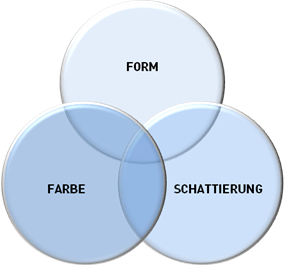
\includegraphics[scale=1.0]{images/Abbildung2.png}
\end{figure}

\begin{itemize}
\item \textbf{Vergessen Sie nicht Ihre Unterschrift unter die Eidesstattliche Erklärung!} Kontrollieren Sie sicherheitshalber jedes Exemplar vor der Abgabe! 
\item Kontrollieren Sie die \textbf{Vollständigkeit} der Exemplare! Achten Sie darauf, dass sich die Formatierung aufgrund von unterschiedlichen Druckern (Ihr Drucker und der Drucker im Copy-Shop) ändern kann. 
\item \textbf{Anzahl einzureichender identischer Exemplare:} zwei 
\end{itemize}